\rcsInfo $Id: cvs-server.tex,v 1.12 2002/12/28 18:43:33 brucker Exp $

\chapter{Excursion: Modeling the Architectures of CVS-server}
In this section, we will discuss several alternatives of CVS-server\index{CVS-server}
architectures, namely the (traditional) closed CVS-server architecture and our
proposed open CVS-server architecture.  The closed CVS-server architecture
naturally arises, if one wishes to install a CVS repository ``out-of-the-box'' but
wants to prevent that users may directly access and destroy the repository;
moreover, if one wants to implement a hierarchical access structure within the
elements of the repository. As already mentioned, our ``open approach'' attempts
to overcome some limitations of the ``closed approach'' at the price of
\emph{potentially} higher security risks - whose formal proof of irrelevance is
the ultimate goal of this paper. The purpose of this section is to give a wider,
architectural perspective of the system than the data-model used and analyzed in
the next sections.

In order to describe the \emph{architecture}\index{architecture} of a
system, it is common practice to use diagrams for this purpose,
enriched by outlines of a formal specification in a behavioral
specification language. Following the approaches of
Garlan~\cite{garlan:arch:93,shaw:arch:96}, architectures are composed
by \emph{components}\index{component} and
\emph{connectors}\index{connector}. Components are computational units
that interact via connectors with each other; connectors can be remote
procedure calls, communication protocols or access to shared
variables. Garlan proposes a semantics for these notions in terms of
the process-algebra CSP~\cite{roscoe:csp:98}\index{CSP}. As a basis for
discussions over the architecture of CVS--server, we will roughly
follow this approach; in this setting, components are just processes,
while connectors are also processes or particular parallel operators
of CSP.

The \emph{closed CVS-server architecture}\index{CVS-server!closed}
is easily depicted as in Fig.~\ref{fig:overview1}.
  \begin{figure}
    \center
      \scalebox{0.5}{\input{pics/arch_overview}}
    \caption{An overview of the standard security architecture.\label{fig:overview1}}
  \end{figure}
In this architecture, we have:
\begin{itemize}
 \item two types of components, (one family of client components, one CVS-server).
 \item client components have two distinct roles (stduser, cvsadmin).
   The standard user gets access along a predefined hierarchy of
   access control rights for the commands \cvscmd{checkin} and
   \cvscmd{checkout}.  The cvs-administrator may additionally change
   the state of the repository by changing the access permissions
   within the repository. The authentication\index{authentication} is
   done in this model by the CVS \cvscmd{login} operation.
 \item the underlying assumption that the repository is internal 
       in a particular closed machine with the repository inside.     
 \item no direct access to the repository by the user,
       only indirect access to the repository by the cvs administrator.
 \item direct access to the repository for the administrator.
\end{itemize}
  \begin{figure}
    \center
      \scalebox{0.5}{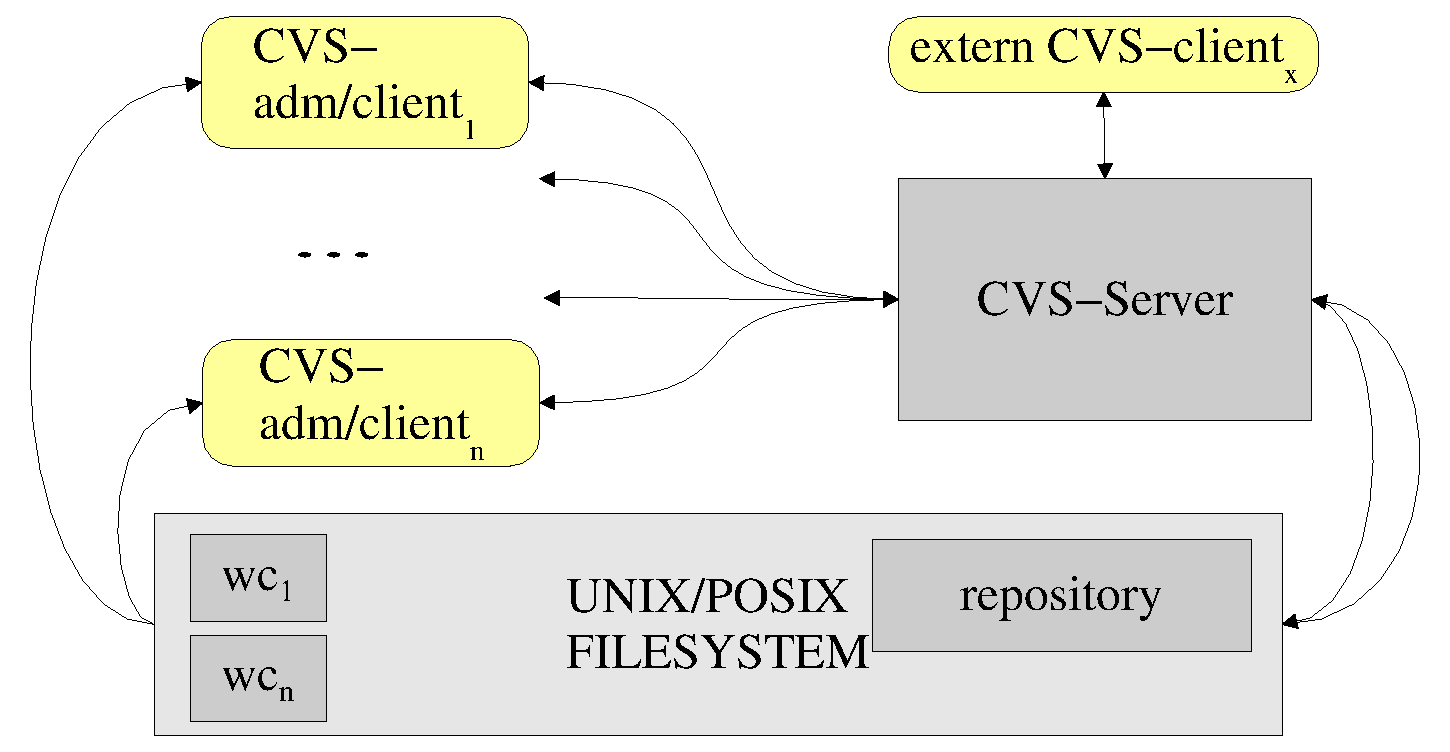
\includegraphics{pics/arch_overview3}}
      \caption{An overview of the open security architecture.\label{fig:overview3}}
  \end{figure}
  In contrast the the setting discussed above, our \emph{open
    CVS-server architecture}\index{CVS-server!open} (see
  Fig.~\ref{fig:overview3}) is depicted as follows:
\begin{itemize}
\item three types components (a family of clients, a server, and the
  UNIX-filesystem).
\item clients may have one of four roles ({stduser, cvsadmin} $\cross$
  {user, sysadmin}).
\item the repository and the working copies are parts of the same
  underlying filesystem; this captures exactly the implementation
  reality.
\item users and CVS-server have in principle equal rights to access the
  filesystem.
\item direct access to the repository for the administrator
\item the architectural view does not capture the fact that the users
  should have \emph{different} access to the elements of the
  repository.
\end{itemize}    
One could add a further type of client into this architecture, namely
the ``externclient'' that has no direct access to the file system;
this represents users that connect to the server without having an
account in the local network the server operates in. But since this
type of client represents a special case of the clients considered
here (and can thus not introduce new complications with respect to
security), we omit it for simplicity reasons.  So far, we have
presented architectures as a graph of of components (belonging to
certain types), that have ``roles'' and that interact along
``connectors'' (depicted as arcs in the diagrams, whose exact nature
is left open.  A more formal description of the model that captures
the communication events in more detail may look as shown in
Fig.~\ref{fig:overview4}.
  \begin{figure}
    \center 
      \scalebox{0.5}{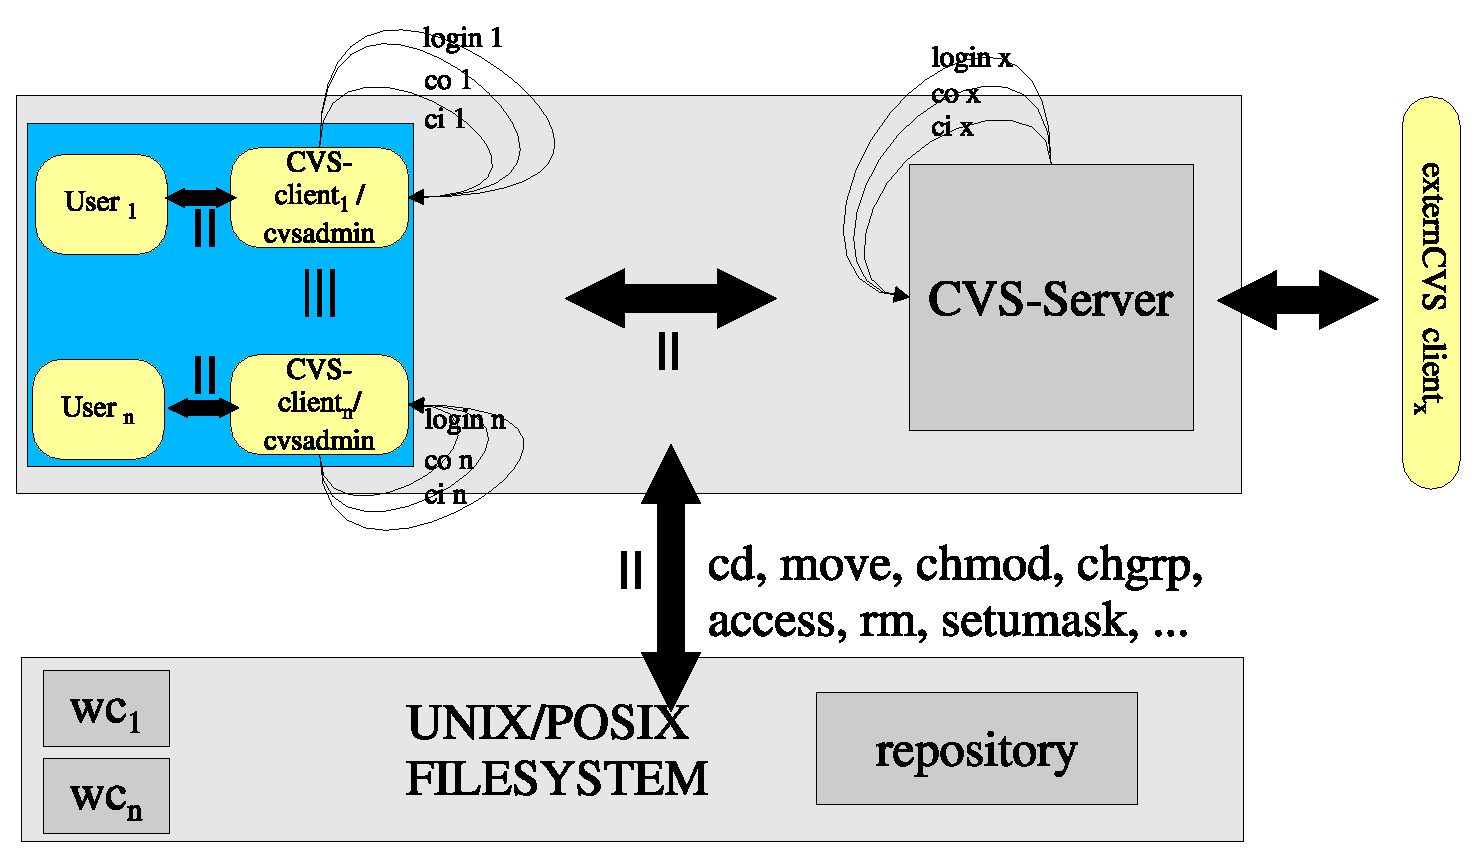
\includegraphics{pics/arch_overview4}}
    \caption{Communication in the open security architecture.\label{fig:overview4}}
  \end{figure}
  Here, we have a collection of user-side CVS-client processes, that may perform
  \cvscmd{cvs\_login}, \cvscmd{cvs\_ci} (checkin), \cvscmd{cvs\_co} (checkout),
  \unixcmd{cd}, \unixcmd{read}, \unixcmd{write}, \unixcmd{mv}, \unixcmd{mkdir},
  \unixcmd{rmdir}, \unixcmd{rm}, \unixcmd{setumask}, \unixcmd{chgrp} and
  \unixcmd{chmod} commands (parameterized in this very simple behavioral model
  just by their user ID $uid$). We assume one particular uid ``root''.  Further,
  we assume a collection of roles and authentication for them.  Now our formal
  architecture model is defined as a collection of interleaved processes that can be
  stated as follows:
\begin{cspverb}
   CLIENT(uid) = |~| role:ROLE,pwd:PWD @ 
                     cvs_login!uid!role!pwd -> CLIENT(uid) |~| 
                     cvs_ci!uid             -> CLIENT(uid) |~|  
                     cvs_co!uid             -> CLIENT(uid) |~|  
                     cd!uid                 -> CLIENT(uid) |~|  
                     read!uid               -> CLIENT(uid) |~|  
                     write!uid              -> CLIENT(uid) |~|  
                     mv!uid                 -> CLIENT(uid) |~| 
                     mkdir!uid              -> CLIENT(uid) |~|  
                     rmdir!uid              -> CLIENT(uid) |~|  
                     rm!uid                 -> CLIENT(uid) |~| 
                     setumask!uid           -> CLIENT(uid) |~|  
                     chgrp!uid              -> CLIENT(uid) |~|  
                     chmod!uid              -> CLIENT(uid) 

   CLIENTS = ||| u:UID @ login!uid -> CLIENT(uid)
\end{cspverb}
In the model above, we allow the user to apply for arbitrary roles ---
later, more refined models of the CVS-server will refuse traces
where the clients do not apply appropriate authentication, but
here we concentrate just on the possible communications. However,
we require that any client process starts with an overall
login command that authenticates the client wrt.\ to the UNIX/Filessystem.

We turn now to the next component, the CVS--server.
It is build as a simple component that accepts all 
logins, checkins   and checkouts, does have (internal) communication with the
file system, and is put into communication with the \texttt{CLIENTS}-component:
\begin{cspverb}
   CVS      = cvs_login?uid  -> CVS []  
              cvs_ci?uid     -> CVS []
              uid            -> CVS []  
              read!cvsadmin  -> CVS []  
              write!cvsadmin -> CVS []  
              mv!cvsadmin    -> CVS [] 
              mkdir!cvsadmin -> CVS []  
              rmdir!cvsadmin -> CVS []  
              rm!cvsadmin    -> CVS

   CLIENTS_CVS = CLIENTS [| {|cvs_login,cvs_ci,cvs_co|} |] CVS
\end{cspverb}
We conclude by putting the whole architecture together with the UNIX-file-
system, which is essentially a server for the \texttt{CLIENTS\_CVS} subsystem.
\begin{cspverb}
   FS    =    login?uid     -> FS [] 
              cd?uid        -> FS []  
              read?uid      -> FS []  
              write?uid     -> FS []  
              mv?uid        -> FS [] 
              mkdir?uid     -> FS []  
              rmdir?uid     -> FS []  
              rm?uid        -> FS [] 
              setumask?uid  -> FS []  
              chgrp?uid     -> FS []  
              chmod?uid     -> FS 

   SYSTEM = CLIENTS_CVS 
              [| {|cd,read,write,mv,mkdir,rmdir,rmdir,rm,
                 setumask,chgrp,chmod|}|] 
            FS
\end{cspverb}
This represents a quite precise view of the possible traces of the system.
However, in principle, the following aspects are not covered by the 
architectural view discussed so far:
\begin{itemize}
    \item The filesystem is a passive listener; its internal state
          is not modeled. In particular it does not contain files
          and their attributes,
    \item therefore, there are no control of reads and writes: 
          the whole UNIX security service is missing.
    \item The architecture does not include ACL-lists,
          we will deliberately not treat this feature of
          our actual implementation in this paper for
          simplicity reasons.
    \item So far, we can not even state security properties \ldots 
    \item nor the security state of repository (ACL's, passwd, file attributes)
    \item the roles and the role changes of the user
\end{itemize}
Since an analysis of the CVS-server security architecture is the main
goal in this paper, we will have to model the compound state of
\texttt{SYSTEM} in more detail. Since the compound state is inherently
complex and requires mostly data structures, their composition and an
overall transition relation over this, and since the communication
aspects of our problem are of minor importance and can be captured on
the level of the trace model of CSP (see~\cite{roscoe:csp:98}), we
will apply in the next sections another specification formalism that
is more suited for this problem domain: namely Z. In particular, tool
support for a wealth of infinite data types (lists, tables, sets,
\ldots) and infinite state models is available, while analysis tools
for CSP\index{CSP} such as FDR\index{FDR} are restricted to finitely
(and small) states and finite data structures.

The formal specification language
Z~\cite{spivey:z_notation:1992}\index{Z} is based on typed set theory
and first-order logic with equality, for which many excellent
textbooks are available (cf.~\cite{woodcock.ea:using:1996}). The
syntax and the semantics are specified in an ISO-standard~\cite{iso:z:2000};
for future standardization efforts of operating system libraries or
programming language semantics, Z is therefore a likely candidate. Z
provides constructs for structuring and combining data-oriented
specifications: schemas model the states of the system (\emph{state
  schemas}\index{schema!state}) and operations on states
(\emph{operation schemas}\index{schema!operation}), while the
\emph{schema calculus}\index{schema calculus} is used to compose these
sub-specifications to larger ones.

We introduce into Z and present these constructs using a standard example,
Spivey's ``birthday book''.  This simple system stores names and dates of
birthdays and provides, for example, an operation to add a new birthday.  In Z,
abstract types for $NAME$ and $DATE$ can be declared that we use in a schema
(consisting of a declaration part and a predicate part) to define the system
state $BirthdayBook$.  For transitions over the system state, the schema
$AddBirthday$ is used:
\begin{zedgroup}
  \begin{schema}{BirthdayBook}
    known: \power NAME \\
    birthday: NAME \pfun DATE \\
    \where
    known = \dom birthday \\
  \end{schema}
  \begin{schema}{AddBirthday}
    \Delta BirthdayBook \\
    n?: NAME; d?: DATE
    \where
    n? \notin known \\
    birthday' = birthday \cup \{n? \mapsto d?\} \\
  \end{schema}
\end{zedgroup}
$\Delta BirthdayBook$ imports the state schema into the operation schema in a
``stroked'' and a ``non-stroked'' version: $BirthdayBook'$ and
$BirthdayBook$. The resulting variables $birthday'$ and $birthday$ are conventionally
understood as the states after and before the operation, respectively.

This system is refined to a more concrete one based on a state $BirthdayBook1$
containing two (unbounded) arrays and an operation that implements $AddBirthday$
on this state:
\begin{zedgroup}
\begin{schema}{BirthdayBook1}
  names: \nat \pfun NAME \\
  dates: \nat \pfun DATE \\
  hwm: \nat \\
  \where
  \forall i,j: 1 \upto hwm @  i \neq j \\
  \t1 \implies names(i) \neq names(j) \\
\end{schema}
\begin{schema}{AddBirthday1}
  \Delta BirthdayBook1 \\
  name?: NAME;  date?: DATE \\
  \where
  \forall i: 1 \upto hwm @ name? \neq names(i) \\
  hwm' = hwm + 1 \\
  names' = names \oplus \{ hwm' \mapsto name? \} \\
  dates' = dates \oplus \{ hwm' \mapsto date? \}
\end{schema}
\end{zedgroup}
One can use the schema calculus to combine different operation schemas into one
operation.  For example, one could strengthen the $AddBirthday$ operation with
an operation schema $AlreadyKnown$ which expresses the fact that the entry that
should be added already exists in the birthday book:
\[
  Add \equiv AddBirthday \lor AlreadyKnown \\
\]
This concludes the birthdaybook-example.

The question arises how architectural --- and this means behavioral
--- descriptions can be formalized in Z, which is traditionally
considered as a data-oriented specification formalism. One part of the
answer is that the \emph{traditional use} of Z is geared toward
data-specifications, the formalism itself is actually powerful enough
to capture both facets of a system: Operation
schemas\index{schema!operation} can be converted into \emph{relation
  on states}, over which traditional transitive closure or trace set
constructions as in the semantics of CSP can be done. Over these,
usual temporal reasoning (is there a state reachable in which a
predicate $P$ holds? If one reaches a state in which $Q$ holds, is it
possible to reach from there a state in which $R$ holds? etc.)
Another part of the answer is concerned with the communication
primitives (e.g. \verb+c!a -> P+ or \verb+c?x -> P x+ in CSP) and
their representation in Z in general and with the representation of
connectors and their representation in our models in particular.  In
general, CSP offers the concept of synchronous communication between
two processes incorporated in the synchronization operator 
\verb+ P [| C |] Q+: if two processes \verb+P+ and \verb+Q+ may engage in an event
$a$ and perform a system transition, that the combined process 
\verb+P [| a |] Q+ may engage in $a$ and result in the combined successor
states of the transition. Such a synchronous communication is a
special form of a connector.  If we represent in Z the transition
relation by an operation schema $P$ and $Q$, we can achieve the effect
of a synchronization as follows, assuming that $P$ sends $a$ to $Q$:
\zcomment{%
\begin{zedgroup}
  \begin{schema}{P}
    \Delta State;
    a : T
    \where
    P_b (x) \\
    a = x \\
  \end{schema}
  \begin{schema}{Q}
    \Delta State;
    a : T
    \where
    Q_b (a) \\
  \end{schema}
\end{zedgroup}
} With the schema calculus\index{schema calculus}, we can now express
the synchronous communication of $P$ to $Q$ via $a$ by a combination
of schema conjunction $\land$ and the hiding operator $\\$
corresponding to existential quantification (which is also the usual
``wiring''-operator between components in hardware design):
\[ PQ \equiv (P \land Q) \setminus \{a\} \; \]
With respect to the logical rules of Z, it is now an easy exercise to
prove that this definition is equivalent to:
\zcomment{%
\begin{zedgroup}
  \begin{schema}{PQ}
    \Delta State
    \where
    P_b (x) \land Q_b (x) \\
  \end{schema}
\end{zedgroup}
}
This logical equivalence motivates how we will use Z with respect to
architectural connectors in particular throughout our specification:
Since we are interested in a ``big-step semantics'' of our system,
i.e.\ $cvs\_add$ will be considered as one big transition step over
the filesystem and intermediate steps (such as internal communication
steps between the client and the server were abstracted away in our model),
we will not distinguish the client and server sides in own schemas.
Instead of introducing an $cvs\_add\_client$ and $cvs\_add\_server$ and putting
them in parallel via synchronization over internal tables to $cvs\_add$,
we will give the specification of the combined system transistions
directly. Alternatively, one could have introduced an own syntax for
architectural compositions; however, since our focus is on theorem
proving and not language design, we consider this approach as out
of the scope of our work. 
%%% Local Variables:
%%% TeX-master: "arch"
%%% fill-column:80
%%% x-symbol-8bits:nil
%%% End:
